\begin{figure}[htbp]
\centering
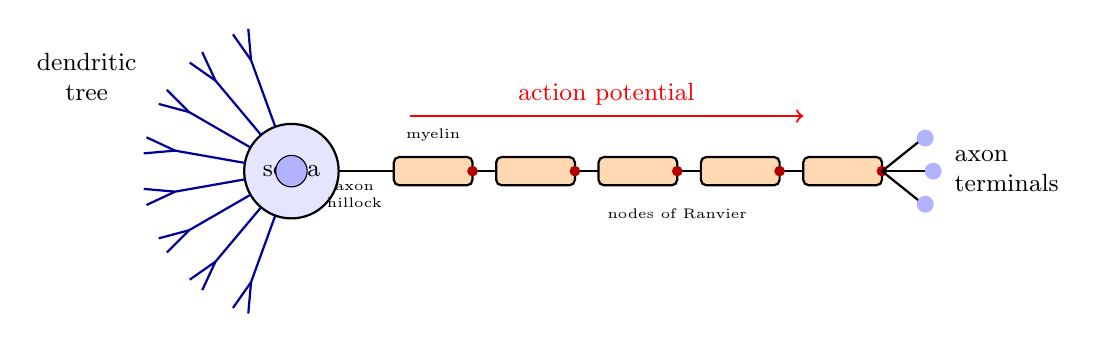
\begin{tikzpicture}[scale=1.0, every node/.style={font=\small}]
  % Soma
  \draw[thick, fill=blue!10] (0,0) circle (0.6);
  \node at (0,0) {soma};
  \draw[fill=blue!30] (0,0) circle (0.2);
  % Dendrites
  \foreach \a in {110, 130, 150, 170, 190, 210, 230, 250} {
    \draw[thick, color=blue!60!black] (\a:0.6) -- ++(\a:0.9);
    \draw[thick, color=blue!60!black] (\a:1.5) -- ++(\a+15:0.4);
    \draw[thick, color=blue!60!black] (\a:1.5) -- ++(\a-15:0.4);
  }
  \node[align=center] at (-2.6,1.2) {dendritic\\tree};
  % Axon hillock
  \draw[thick] (0.6,0) -- (1.0,0);
  \node[below, align=center, font=\tiny] at (0.8,-0.05) {axon\\hillock};
  % Axon with myelin segments
  \draw[thick] (1.0,0) -- (7.5,0);
  \foreach \x in {1.3, 2.6, 3.9, 5.2, 6.5} {
    \draw[thick, fill=orange!30, rounded corners=2pt] (\x,-0.18) rectangle (\x+1.0,0.18);
  }
  \node[above, font=\tiny] at (1.8,0.25) {myelin};
  % Nodes of Ranvier
  \foreach \x in {2.3, 3.6, 4.9, 6.2, 7.5} {
    \filldraw[red!70!black] (\x,0) circle (0.06);
  }
  \node[below, align=center, font=\tiny] at (4.9,-0.35) {nodes of Ranvier};
  % Axon terminals
  \draw[thick] (7.5,0) -- (8.0,0.4);
  \draw[thick] (7.5,0) -- (8.0,-0.4);
  \draw[thick] (7.5,0) -- (8.1,0);
  \filldraw[blue!30] (8.05,0.42) circle (0.1);
  \filldraw[blue!30] (8.05,-0.42) circle (0.1);
  \filldraw[blue!30] (8.15,0) circle (0.1);
  \node[right, align=left] at (8.3,0) {axon\\terminals};
  % Direction arrow
  \draw[->, thick, color=red] (1.5,0.7) -- (6.5,0.7) node[midway, above] {action potential};
\end{tikzpicture}
\caption[Neuron schematic]{Schematic of a vertebrate motor neuron. Dendrites
(left) integrate synaptic inputs; the soma houses the nucleus; the
axon hillock initiates the action potential; the myelinated axon
propagates the spike by saltatory conduction across nodes of Ranvier;
axon terminals release neurotransmitter onto downstream neurons or
muscle.}
\label{fig:vol06:ch07:neuron}
\end{figure}
